%!TEX program = xelatex
\documentclass[12pt,a4paper]{ctexart}

\usepackage[left=2.0cm,right=2.0cm,top=1.6cm,bottom=1.4cm]{geometry}
\usepackage{setspace}
\setstretch{1.05}
\usepackage{booktabs}
\usepackage{graphicx}
\usepackage{cite}
\usepackage{tabularx}
\usepackage{caption}
\usepackage{subcaption}
\usepackage{float}
\usepackage{hyperref}
\usepackage{titlesec}
\titleformat{\section}{\large\bfseries}{}{0em}{}
\titlespacing{\section}{0pt}{6pt}{2pt}
\titleformat{\subsection}{\normalsize\bfseries}{}{0em}{}
\titlespacing{\subsection}{0pt}{4pt}{1pt}
\titleformat{\subsubsection}{\small\bfseries}{}{0em}{}
\titlespacing{\subsubsection}{0pt}{3pt}{1pt}

\graphicspath{{figures/}}

\begin{document}

\title{\vspace{-0.8cm}\textbf{面向生物医学文献的多策略多标签\\
分类方法系统比较研究\\
——以空间转录组学文献自动分类为例}}
\author{李哲夫\quad 2023011400\quad 生32\\[2pt]
\texttt{\footnotesize\url{https://github.com/zf-li23/pubmed-spatial-tracker}}}
\date{}
\maketitle
\vspace{-0.6cm}

\begin{abstract}
\small
生物医学文献呈指数增长，自动多标签分类面临文本稀疏、标签空间复杂和标注成本高等多重挑战。
本文构建了一个\textbf{多数据集~$\times$~多算法~$\times$~多特征表示}的系统性实验框架，
在四个独立数据集（OHSUMED、PubMed-MultiLabel、PGB、自建空间转录组学文献库）上，
系统比较了\textbf{5~种文本表示、14~种分类算法和3~种多标签策略}，
共完成\textbf{7~组实验、113/115~子任务（98.3\%）}。
核心发现如下：(1)~BioBERT 嵌入在所有数据集上系统性优于 TF-IDF，提升 10--30\%；
(2)~标签密度决定算法排序——稠密标签场景 Logistic~Regression 最优，极稀疏标签场景 AdaBoost 最优；
(3)~图卷积网络（GCN）在节点分类任务上显著优于 Node2Vec 和 GraphSAGE；
(4)~在自建空间转录组学文献库上，BioBERT+MLP 达到 F1=0.8444；
(5)~通过 PubMed-MultiLabel 预训练后微调，F1 进一步提升至 \textbf{0.9143}（+9.6\%），
验证了“宽泛预训练~+~领域微调”范式的有效性。
\end{abstract}

% ═══════════════════════════════════════════════════════════════
\section{一、引言}
% ═══════════════════════════════════════════════════════════════

生物医学文献正以指数速度增长。以空间转录组学（Spatial Transcriptomics）领域为例，
PubMed 年发文量从 2020 年以前不足 500 篇激增至 2025 年的 4,150 篇，
传统人工分类已完全不可行。自动文献分类面临三重挑战：
(1)~\textbf{文本稀疏}——词袋模型无法捕捉医学术语间的语义关联（如“心肌梗塞”与“冠心病”）；
(2)~\textbf{标签空间复杂}——一篇文献可能同时涉及研究类别、技术平台、分析方法和生物学领域，
构成天然的多标签问题；
(3)~\textbf{标注成本高}——大规模人工标注需要领域专家，时间和经济成本极高。
BioBERT\footnote{Lee et al., Bioinformatics, 36(4), 2020} 等预训练语言模型在生物医学文本挖掘中取得了显著成功，
PGB\footnote{Lee \& Ho, arXiv:2305.02691, 2023} 进一步将图神经网络引入生物医学文献理解，
而 BioCreative VII LitCovid Track\footnote{Chen et al., Database, 2022} 等评测任务则推动了多标签文献分类的标准化评估。
Biomed-Enriched\footnote{Touchent et al., arXiv:2506.20331, 2025} 提出的两阶段 LLM 标注方法
为大规摸文献标注提供了新的低成本途径。

针对上述挑战，本文设计了\textbf{多数据集~$\times$~多算法~$\times$~多特征表示}的系统性比较框架，
回答以下核心研究问题：
\begin{itemize}
  \setlength{\itemsep}{-1pt}\setlength{\parsep}{0pt}
  \item 不同算法在不同标签粒度下的性能排序是否一致？
  \item 图结构信息对文献分类有无边际收益？
  \item 大语言模型（LLM）批量标注能否替代人工标注？
  \item “宽泛预训练~+~领域微调”的迁移学习范式是否有效？
\end{itemize}

% ═══════════════════════════════════════════════════════════════
\section{二、数据集}
% ═══════════════════════════════════════════════════════════════

本文使用四个独立数据集，从标签粒度、信息维度和标注完备性三个维度形成天然梯度
（表~\ref{tab:datasets}）。

\begin{table}[htbp]
\centering
\caption{四个数据集对比}
\label{tab:datasets}
\small
\begin{tabular}{cccccc}
\toprule
\textbf{数据集} & \textbf{规模} & \textbf{标签数} & \textbf{标签类型} & \textbf{标注方式} & \textbf{角色} \\
\midrule
OHSUMED       & $\sim$10K 篇 & 1,650 & MeSH 多标签 & 人工 & 稀疏标签基准 \\
PML           & 10K 篇       & 16    & 顶级类别     & 人工 & 粗粒度实验   \\
PGB           & 5K 篇        & 3     & 节点分类     & 人工 & 图方法验证   \\
Spatial Tracker & 9,148 篇  & 40+   & 多维标签     & LLM  & 目标应用     \\
\bottomrule
\end{tabular}
\end{table}

\textbf{OHSUMED}\footnote{\url{https://trec.nist.gov/data/filtering/t9.filtering.tar.gz}}
来自 TREC-9 Filtering Track，包含 1987--1991 年间的 MEDLINE 文献摘要，
标注有 14,466 个 MeSH 词（经低频过滤保留 1,650 个），标签呈典型幂律分布。
该数据集用于评估算法在极稀疏多标签场景下的性能。
\begin{figure}[H]
\centering
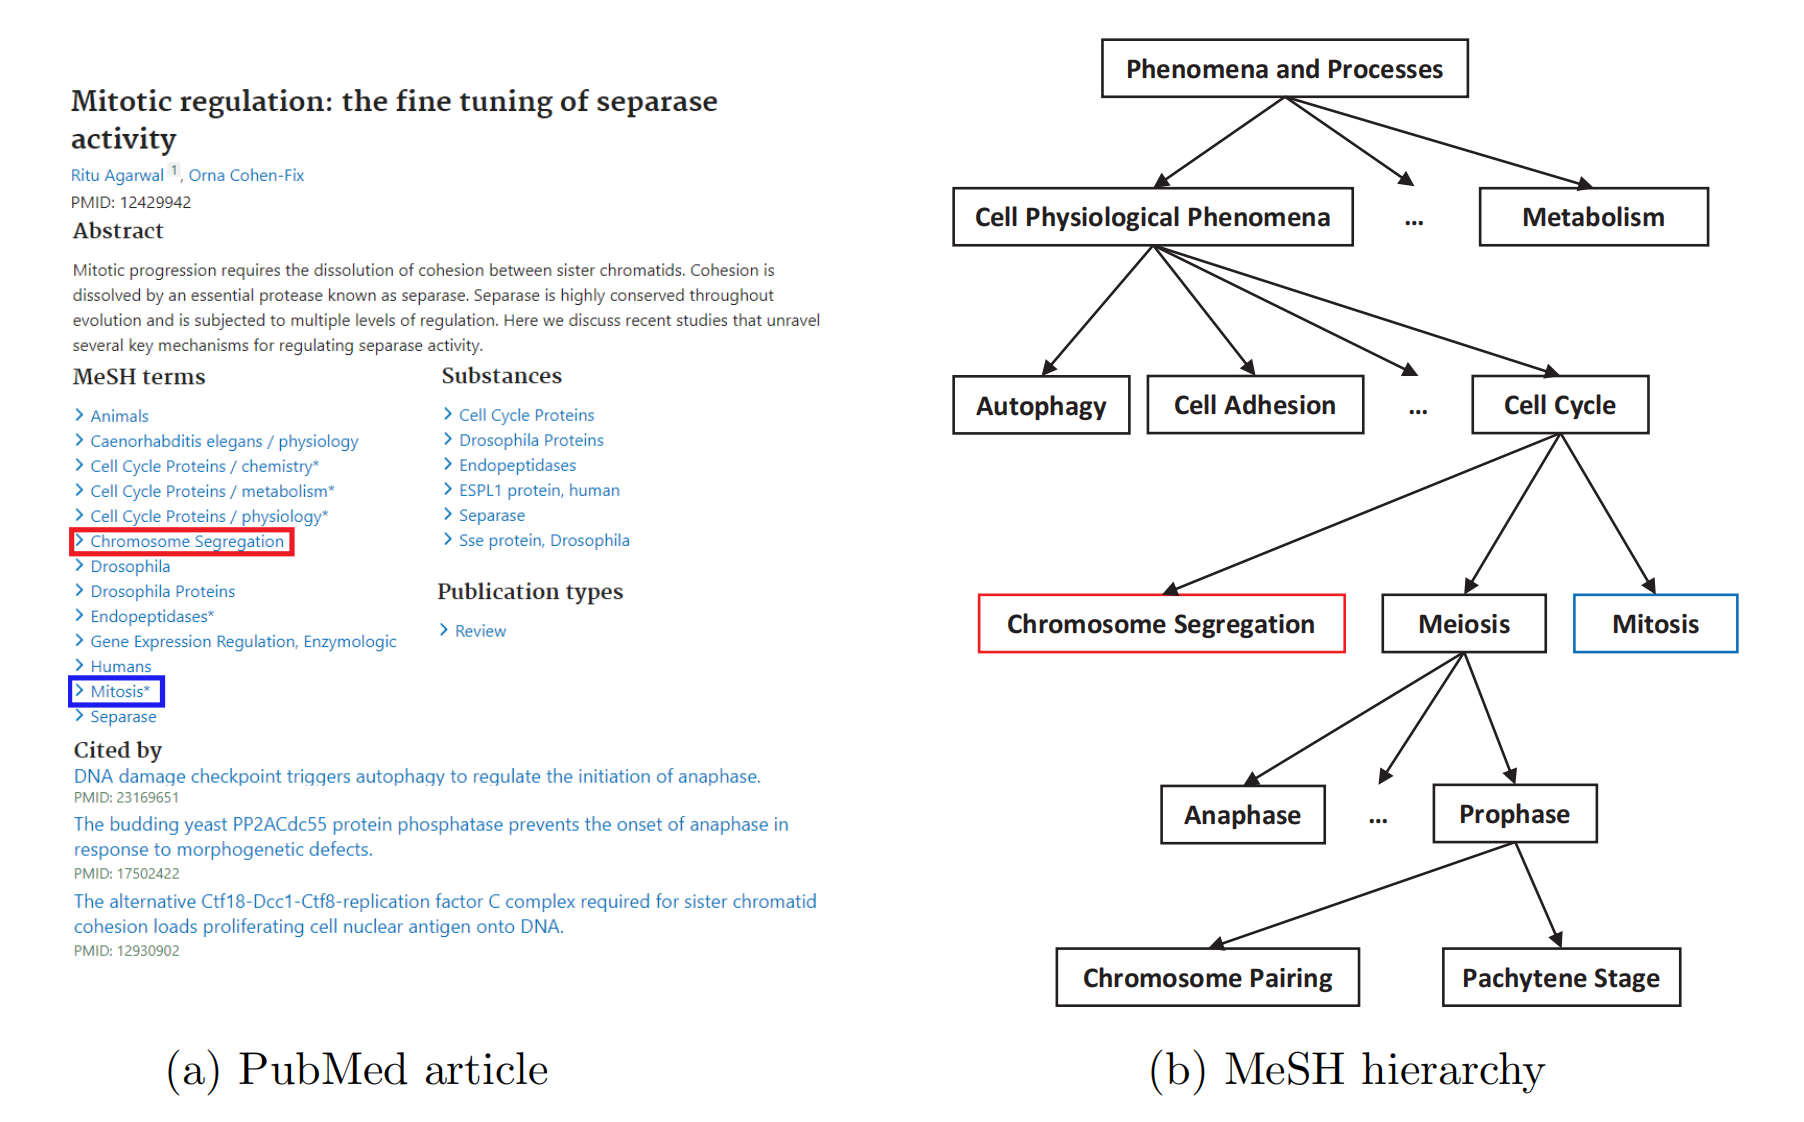
\includegraphics[width=0.82\textwidth]{image0.png}
\caption{PubMed 文章及其关联的 MeSH 层级结构示例\protect\footnotemark。
（a）一篇 PubMed 文章包含标题、摘要、引用列表、发表类型、MeSH 词和物质列表；
（b）MeSH 层级树将 MeSH 词归类到更宽泛的概念之下。}
\label{fig:mesh}
\end{figure}
\footnotetext{图片来自 Lee \& Ho, arXiv:2305.02691, 2023 Figure~1。}
\textbf{PubMed-MultiLabel (PML)}\footnote{\url{https://www.kaggle.com/datasets/owaiskhan9654/pubmed-multilabel-text-classification}}
包含 10K 篇文献，标注有 15 个 MeSH 顶级类别（另加 Other 类共 16 类）。
数据干净、标签稠密，适合快速算法筛选。

\textbf{PGB (PubMed Graph Benchmark)}\footnote{Lee \& Ho, arXiv:2305.02691, 2023}
是包含 $\sim$30M 篇论文及其引用关系的异构图数据集。
本文采样 5K 篇并引用其 3 类节点分类任务，用于验证图表示学习方法。

\textbf{Spatial Tracker (ST)} 是本文自建的数据集。
通过以下 PubMed 检索式爬取并筛选得到 9,148 篇空间转录组学相关文献：
{\small\begin{verbatim}
("Spatial Transcriptomics"[MeSH Major Topic]
 OR "spatial transcriptom*"[Title/Abstract]
 OR "spatially resolved transcriptom*"[Title/Abstract])
AND hasabstract[text] AND english[Language]
AND 2016:2026[dp]
\end{verbatim}}
参考 Biomed-Enriched 方法\footnote{Touchent et al., arXiv:2506.20331, 2025}，
使用 DeepSeek-v4-flash 大语言模型设计了包含 6 个类别、15 个分析标签、
19 个技术平台和 17 个生物学领域的多维标签体系，完成了全部 9,148 篇的批量标注。
标注结果显示：Research 类占 58.3\%，Technology 占 19.5\%，Review 占 14.3\%，
高置信度和中置信度合计占 95.6\%。

\begin{figure}[htbp]
\centering
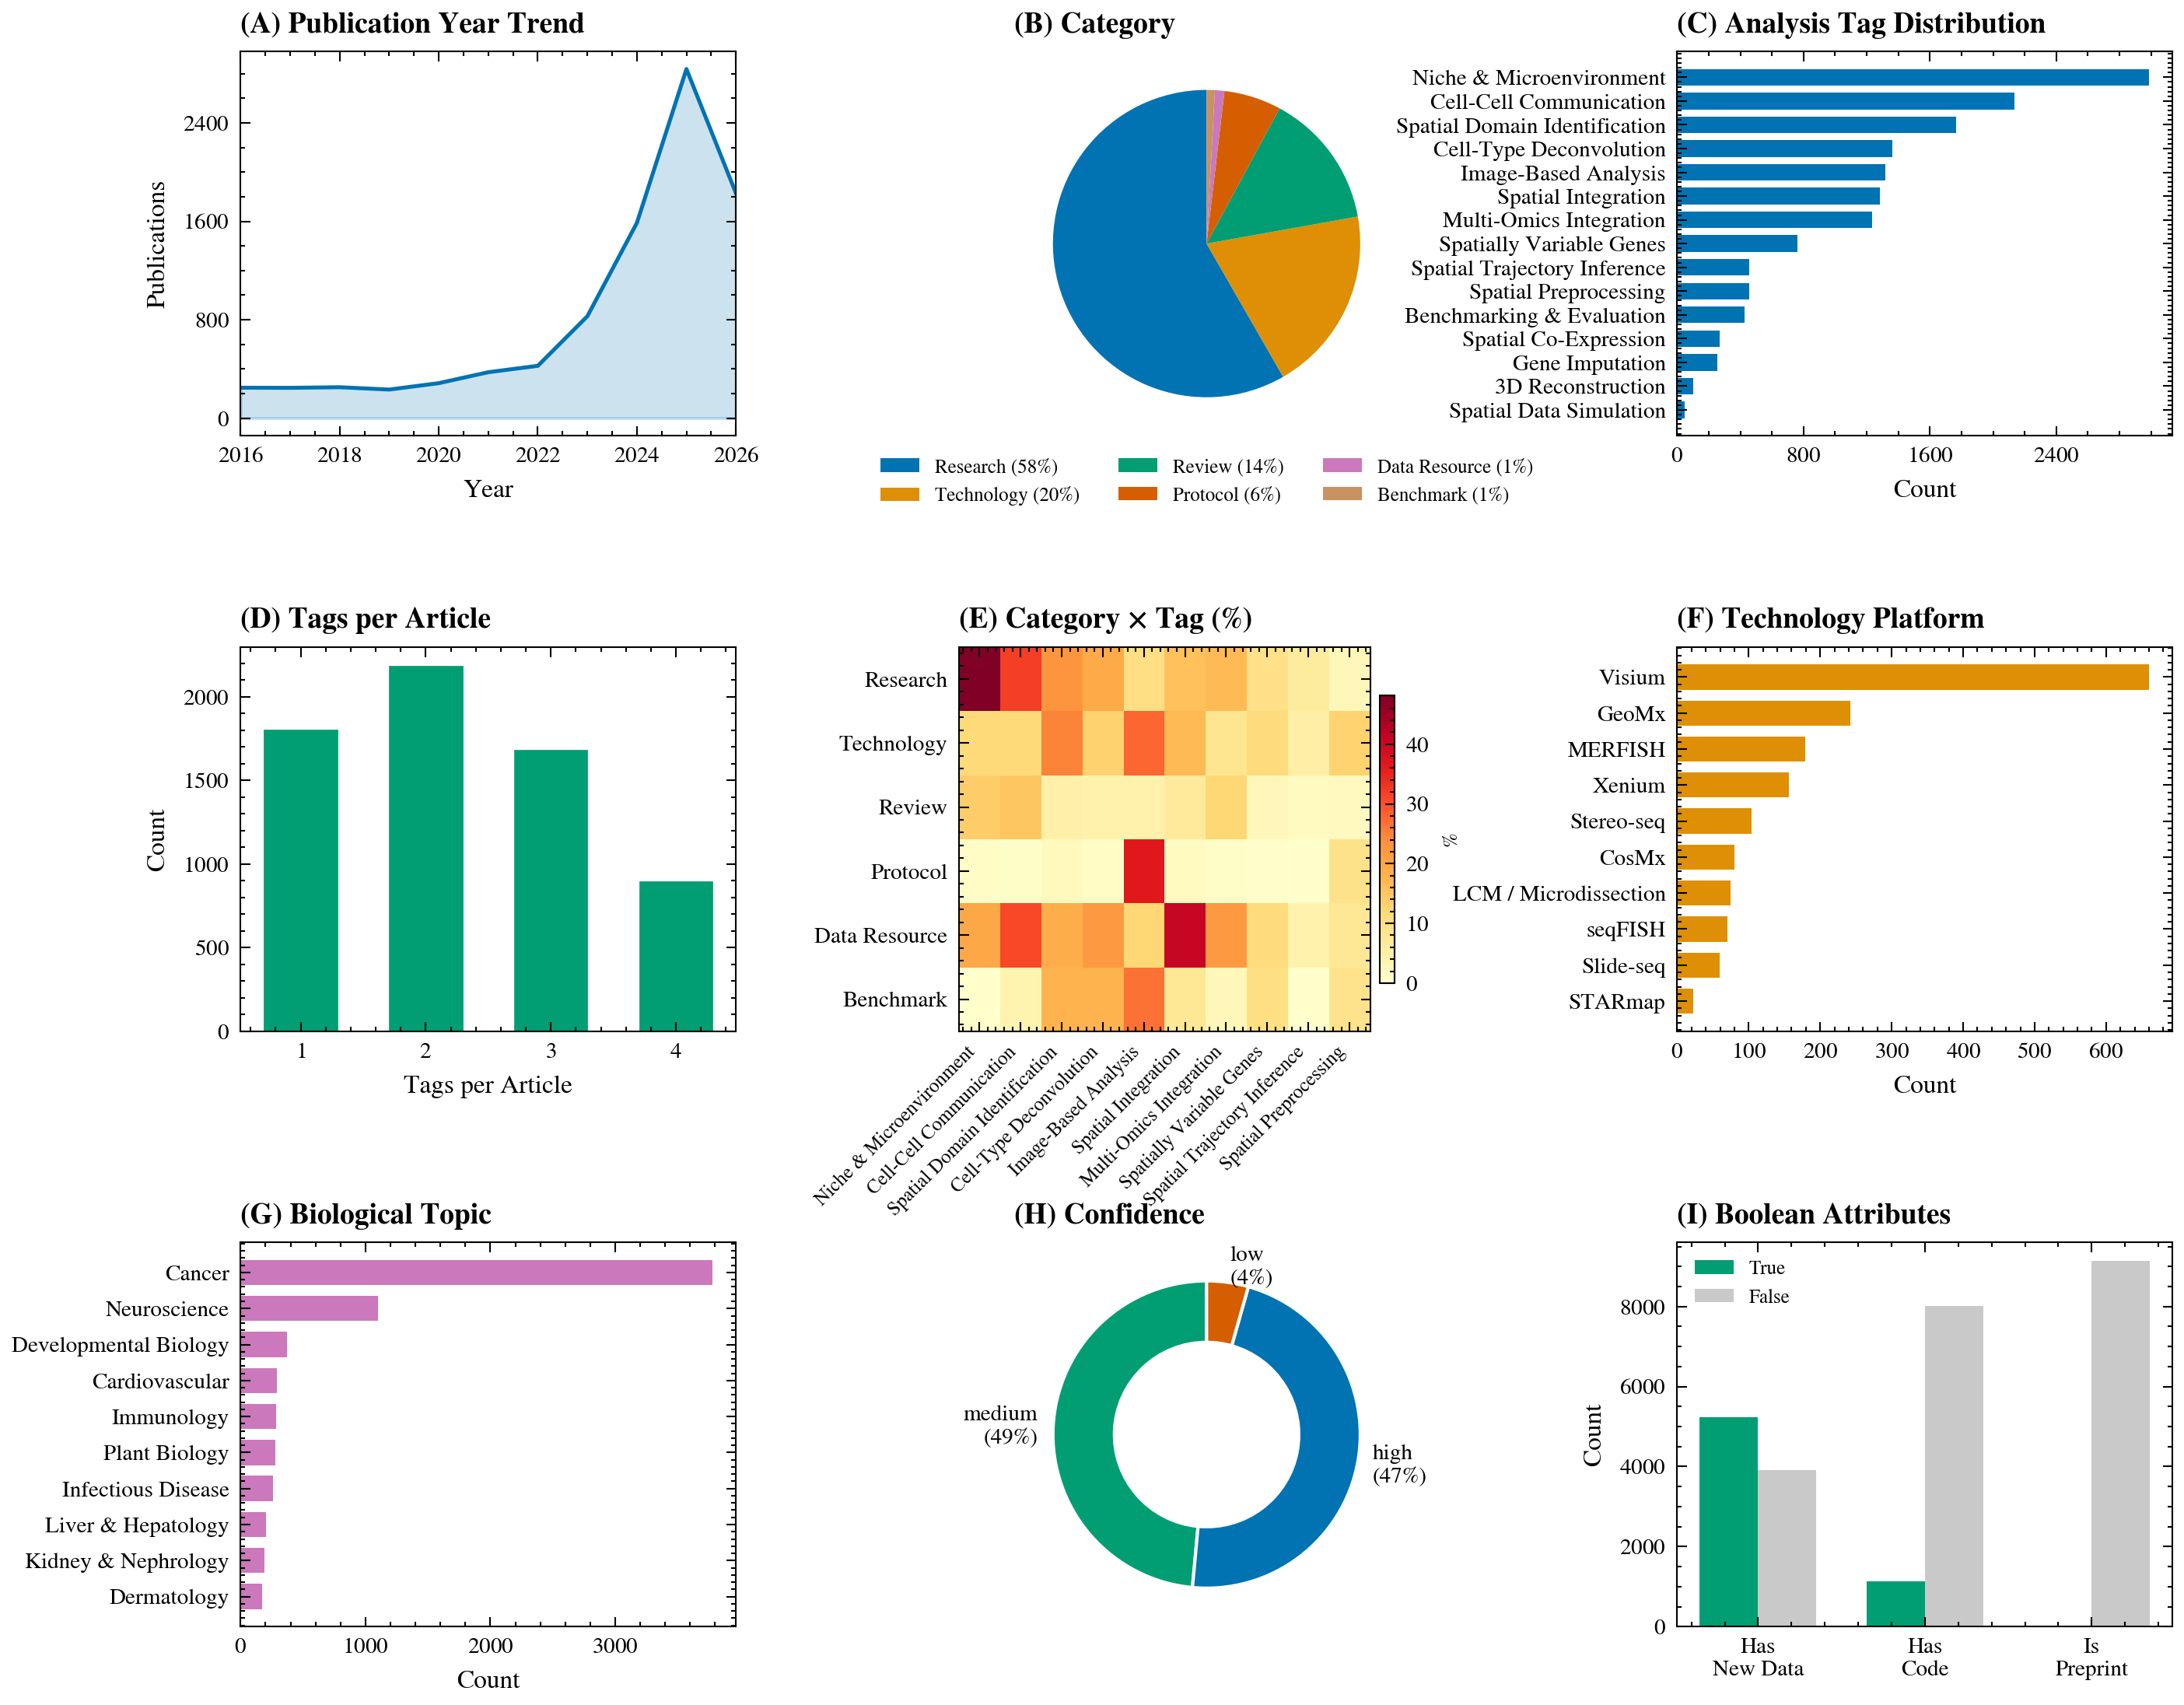
\includegraphics[width=\textwidth]{fig1_dataset_overview.png}
\caption{数据集概览。（A）年度发文趋势；（B）类别饼图；（C）分析标签分布（Top~15）；
（D）每篇文章标签数直方图；（E）类别~$\times$~标签热力图（\%，行归一化）；（F）技术平台分布（Top~10）；
（G）生物学主题分布（Top~10）；（H）标注置信度环形图；（I）布尔属性（has\_new\_data~/~has\_code~/~is\_preprint）。}
\label{fig:overview}
\end{figure}

% ═══════════════════════════════════════════════════════════════
\section{三、方法}
% ═══════════════════════════════════════════════════════════════

\subsection{文本表示}

文本分类的基本流程包括数据预处理、特征提取、模型训练和评估等步骤
（图~\ref{fig:tcsteps}）。

\begin{figure}[H]
\centering
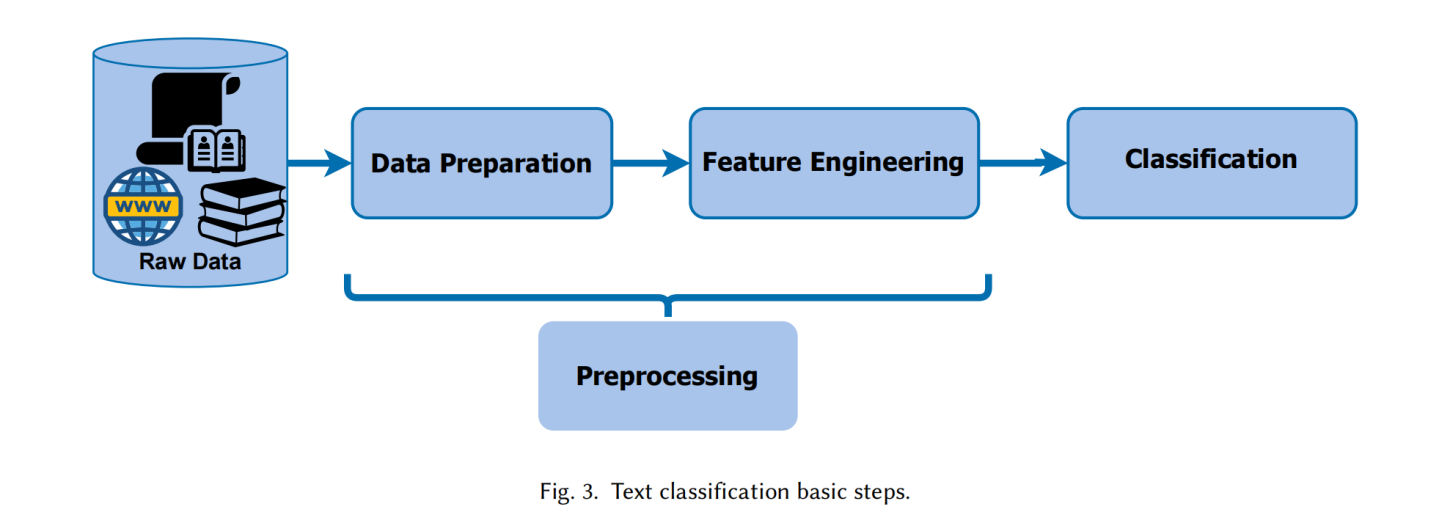
\includegraphics[width=0.75\textwidth]{image1.png}
\caption{文本分类基本步骤\protect\footnotemark。}
\label{fig:tcsteps}
\end{figure}
\footnotetext{图片来自 Rostam \& Kert\'{e}sz, ACM TIST, 2025, Figure~3。}

本文采用 5 种互补的文本表示方法，从不同粒度和维度捕捉文献语义：

\begin{itemize}
  \setlength{\itemsep}{-1pt}\setlength{\parsep}{0pt}
  \item \textbf{TF-IDF}（1--2~gram, max\_features=5,000）：词级稀疏特征，
  可解释性强，作为经典基线。
  \item \textbf{BioBERT}（\texttt{dmis-lab/biobert-base-cased-v1.1}，
  mean~pooling 至 768 维）：在 PubMed 摘要和 PMC 全文上预训练的语言模型，
  能捕捉医学术语的上下文语义关系。
  \item \textbf{LDA}（$K=15$）：文档级主题分布，捕捉隐式主题结构。
  \item \textbf{元特征}（出版年份、文本长度等 3--5 维）：非文本信号，辅助分类。
  \item \textbf{Node2Vec}（128 维）：仅在 PGB 上使用，在有偏随机游走中
  学习文献节点的图结构嵌入。
\end{itemize}

\subsection{分类算法}

共实现 14 种分类算法，覆盖课程全部主要模块（表~\ref{tab:algorithms}）。

\begin{table}[htbp]
\centering
\caption{分类算法一览}
\label{tab:algorithms}
\small
\begin{tabular}{cll}
\toprule
\textbf{课程模块} & \textbf{算法} & \textbf{数量} \\
\midrule
贝叶斯学习       & Naive Bayes (GaussianNB)         & 1 \\
基于实例的学习   & $k$-NN, SVM (RBF)                 & 2 \\
回归学习         & Logistic Regression               & 1 \\
集成学习 (Bagging)  & Random Forest                   & 1 \\
集成学习 (Boosting) & AdaBoost, XGBoost               & 2 \\
深度学习         & BioBERT + MLP                     & 1 \\
无监督学习       & LDA + KMeans                      & 1 \\
图表示学习       & Node2Vec + 分类器, GCN, GraphSAGE & 5 \\
\midrule
\textbf{合计}   & & \textbf{14} \\
\bottomrule
\end{tabular}
\end{table}

对于多标签任务，额外比较了三种问题转换策略：
\textbf{Binary Relevance}（BR，每个标签独立二分类）、
\textbf{Classifier Chains}（CC，链式传递标签依赖）和
\textbf{Label Powerset}（LP，标签组合转为多分类）。

\subsection{实验设计}

实验采用\textbf{三步渐进}策略：

\textbf{Step~1：多数据集算法筛选。}
在 OHSUMED、PML 和 PGB 三个全标注数据集上，
执行 7 种经典算法~$\times$~4 种特征~$\times$~3 数据集 = 84 组实验（Exp~001），
以及 BioBERT+MLP 端到端微调（Exp~002）、LDA+KMeans 聚类（Exp~003）、
多标签策略对比（Exp~004）和图模型对比（Exp~005），
共 105 组子任务。

\textbf{Step~2：目标数据集构建与应用。}
通过 PubMed 检索构建空间转录组学文献数据集（9,148 篇），
使用 DeepSeek-v4-flash 完成 LLM 批量标注，
然后在 ST 上执行三种方法的基准测试（Exp~006）。

\textbf{Step~3：迁移微调探索。}
在 PML、OHSUMED 和 PGB 上预训练，
在 ST 上微调（Exp~007），量化迁移学习的增益。

所有实验均采用\textbf{5 折交叉验证}，
主要评价指标为 Macro F1，辅以 Accuracy、NMI 和配对 $t$ 检验。

% ═══════════════════════════════════════════════════════════════
\section{四、实验结果}
% ═══════════════════════════════════════════════════════════════

\subsection{Exp~001：经典算法矩阵（84/84 完成）}

7 种模型~$\times$~4 种特征~$\times$~3 数据集共 84 组实验全部完成。
表~\ref{tab:exp001} 展示了各数据集的最佳组合。

\begin{table}[htbp]
\centering
\caption{Exp~001 各数据集最佳组合}
\label{tab:exp001}
\small
\begin{tabular}{clcc}
\toprule
\textbf{数据集} & \textbf{最佳组合} & \textbf{F1-macro} & \textbf{次优组合} \\
\midrule
OHSUMED (1,650~标签) & AdaBoost + TF-IDF & \textbf{0.1687} & LR+BioBERT (0.0853) \\
PML (16~标签)        & LogisticReg + BioBERT & \textbf{0.6710} & SVM+BioBERT (0.6603) \\
PGB (3~类)           & AdaBoost + TF-IDF & \textbf{0.4215} & SVM+TF-IDF (0.3775) \\
\bottomrule
\end{tabular}
\end{table}

\textbf{关键发现}：(1)~BioBERT 嵌入系统性优于 TF-IDF——
在 PML 上 LogisticReg+BioBERT (0.6710) 比最佳 TF-IDF 组合 SVM+TF-IDF (0.5682) 提升 18\%。
(2)~标签密度决定算法排序——在稠密标签 PML 上，Logistic~Regression 表现最佳；
在稀疏标签 OHSUMED 上，AdaBoost 以 0.1687 远超其他模型。
(3)~OHSUMED 的 1,650 个标签过于稀疏，所有模型 F1-macro 均低于 0.2，
说明极多标签场景仍需进一步探索。

\begin{figure}[htbp]
\centering
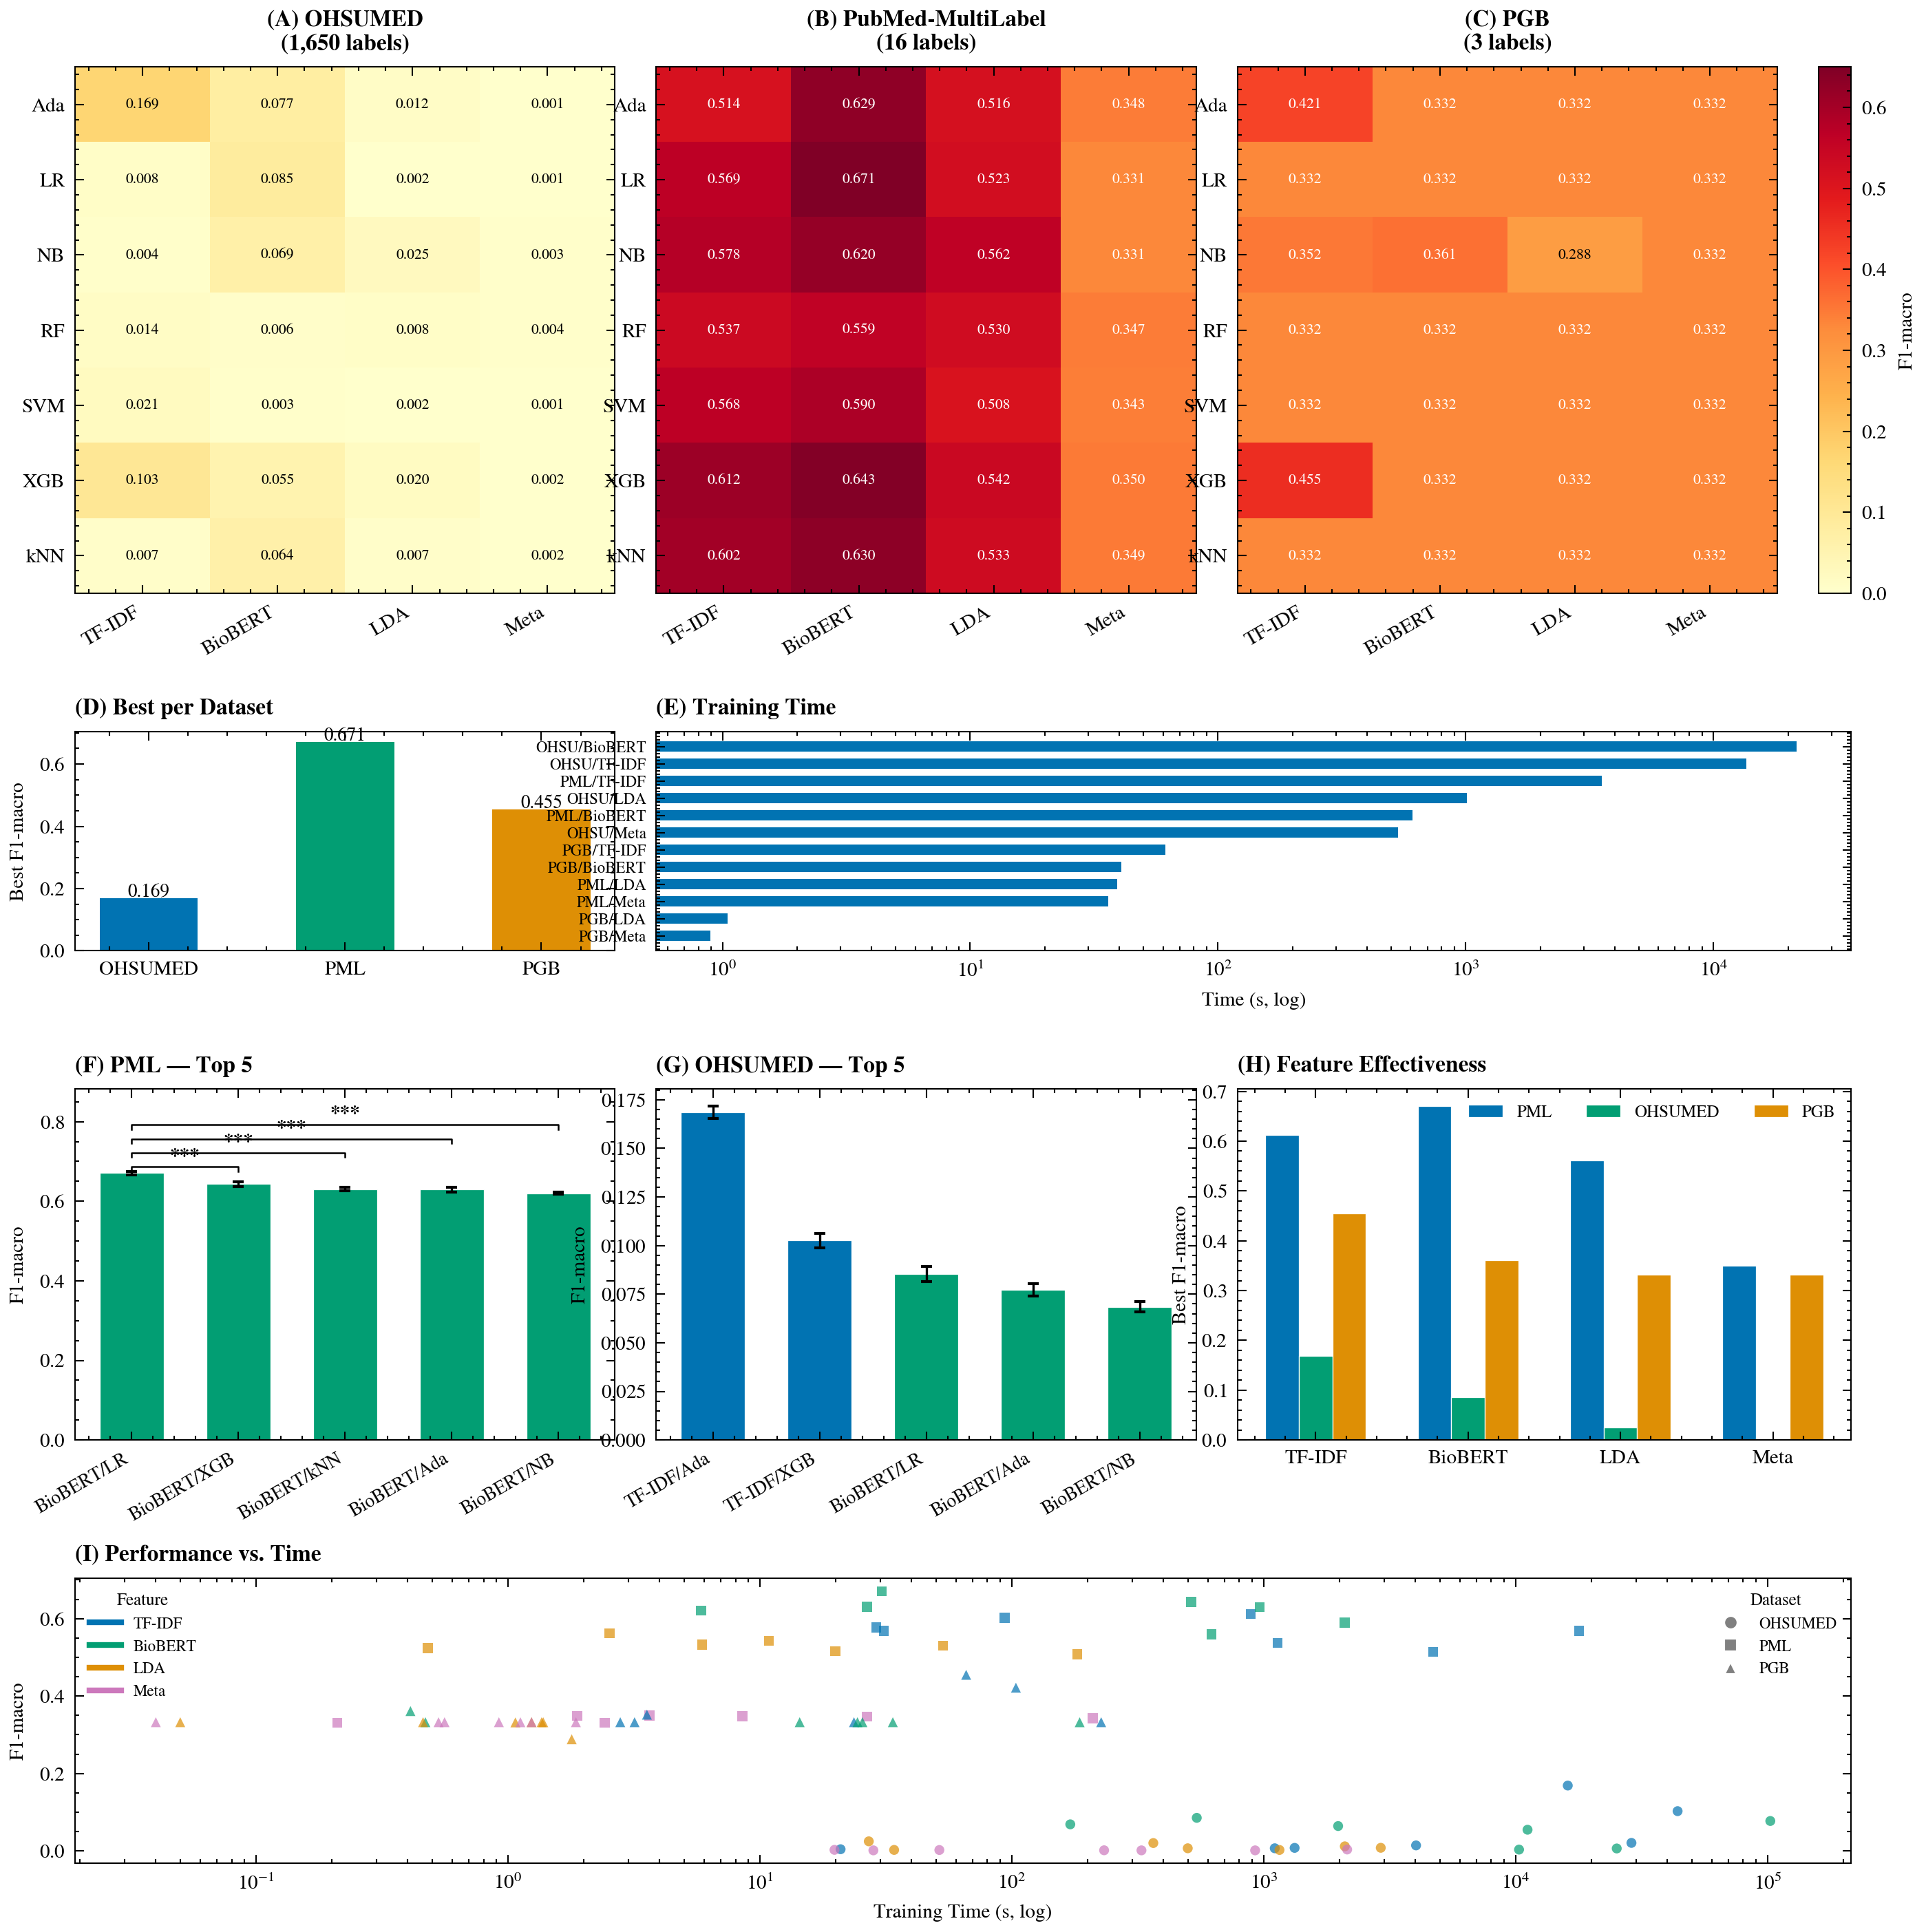
\includegraphics[width=\textwidth]{fig2_classical_matrix.png}
\caption{经典算法矩阵实验结果。（A）OHSUMED 特征~$\times$~模型 F1-macro 热力图；
（B）PML 热力图；（C）PGB 热力图；（D）各数据集最佳 F1-macro 对比；
（E）各组合训练时间对比（对数坐标）；（F）PML Top-5 模型及显著性标注；
（G）OHSUMED Top-5 模型；（H）各特征的最佳 F1-macro 跨数据集对比；
（I）F1-macro 与训练时间的散点图（对数坐标）。}
\label{fig:classical}
\end{figure}

\subsection{\texorpdfstring{Exp~002~$\sim$~004}{Exp 002–004}：BioBERT 微调、无监督聚类与多标签策略}

\textbf{BioBERT+MLP 端到端微调（Exp~002）}显示：
PML 上微调后 F1=0.6411，与冻结 BioBERT 嵌入配合 Logistic~Regression 的 0.6710 接近，
说明端到端微调在粗粒度标签上的增益有限。
OHSUMED 上仅 0.0013（标签太稀疏），PGB 上 0.3601。

\textbf{LDA+KMeans 聚类（Exp~003）}显示：
OHSUMED 的主题结构最清晰（NMI=0.44），
PML 中等（NMI=0.10），PGB 基本不可分（NMI$\approx$0），
这与数据集标签粒度和文档内容的区分度一致。

\textbf{多标签策略对比（Exp~004）}显示：
在 PML（16 标签）上，Classifier Chains 以 F1=0.5796 略优于
Binary Relevance 和 Label Powerset（均为 0.5686），
说明链式传递能捕捉有限的标签依赖关系。
但在 OHSUMED（1,650 标签）上所有策略 F1 均低于 0.01，
标签空间过大时多标签策略失效。

\subsection{Exp~005：图模型}

在 PGB 上比较了 Node2Vec + 6 种分类器、GCN 和 GraphSAGE。
结果如表~\ref{tab:graph} 所示。

\begin{table}[htbp]
\centering
\caption{Exp~005 图模型结果}
\label{tab:graph}
\small
\begin{tabular}{lcc}
\toprule
\textbf{方法} & \textbf{F1-macro} & \textbf{备注} \\
\midrule
GCN            & \textbf{0.4125} & 图卷积结构最优 \\
GraphSAGE      & 0.3324          & 与 Node2Vec 持平 \\
Node2Vec+LR    & 0.3324          & 各分类器结果相近 \\
Node2Vec+SVM   & 0.3324          & \\
Node2Vec+kNN   & 0.3324          & \\
\bottomrule
\end{tabular}
\end{table}

\textbf{GCN 显著优于 Node2Vec 和 GraphSAGE}（0.4125 vs 0.3324），
说明图卷积操作能有效利用邻居节点的特征信息，而随机游走（Node2Vec）
和采样聚合（GraphSAGE）在 PGB 的 5K 子图上未能充分体现优势。
Node2Vec 各分类器的结果基本持平（$\sim$0.3324），
说明嵌入本身的信息量是瓶颈，而非分类器的选择。

\begin{figure}[htbp]
\centering
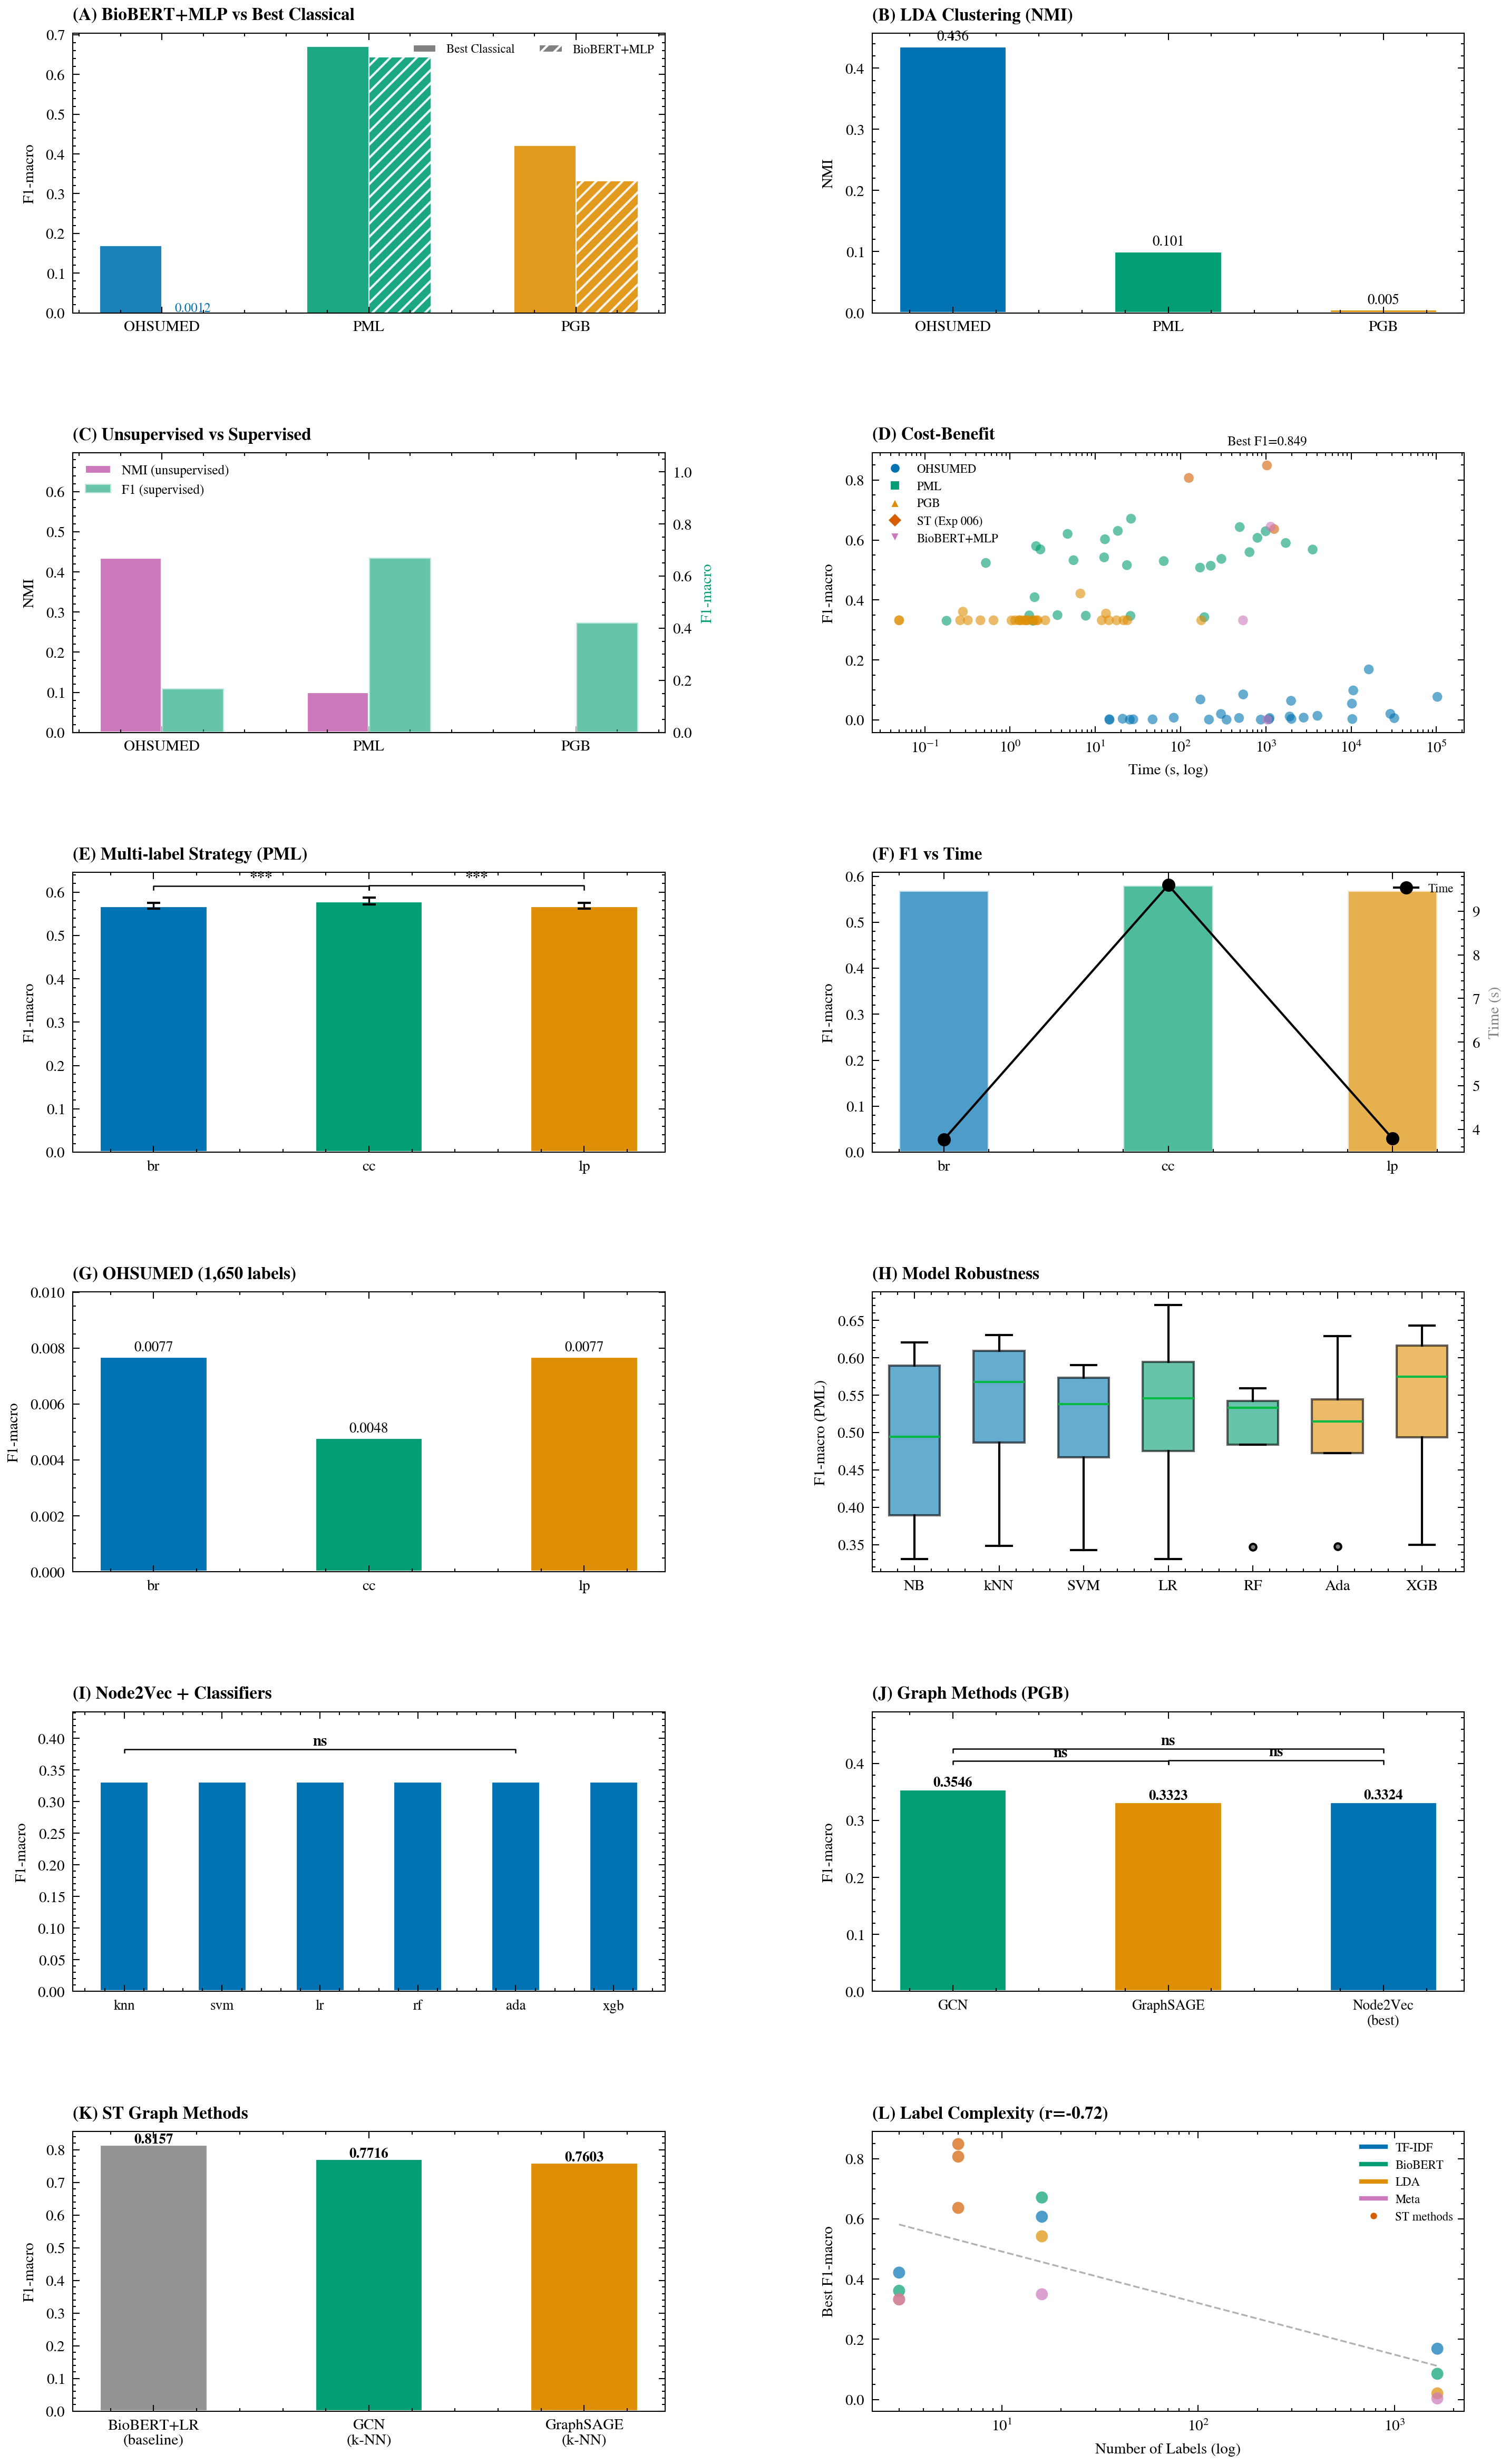
\includegraphics[width=0.82\textwidth]{fig3_unsupervised_multilabel_graph.png}
\caption{无监督学习、多标签策略与图模型实验结果。
（A）BioBERT+MLP vs 最佳经典算法；（B）LDA 聚类质量（NMI）；
（C）无监督 vs 有监督对比；（D）成本-效益散点图（F1 vs 时间）；
（E）多标签策略对比（PML，BR/CC/LP）；
（F）多标签策略 F1 vs 训练时间；（G）OHSUMED 多标签策略（1,650~标签）；
（H）各模型在 PML 上的 F1 箱线图（模型鲁棒性）；
（I）Node2Vec + 各分类器结果及显著性；（J）图方法对比（GCN / GraphSAGE / Node2Vec）；
（K）ST~$k$-NN 图方法（GCN / GraphSAGE vs 基线）；（L）标签复杂度（F1-macro 随标签数变化）。}
\label{fig:unsup}
\end{figure}

\subsection{Exp~006：空间转录组学文献基准测试}

在 ST 数据集（9,148 篇，6 类）上比较三种方法（表~\ref{tab:st}）。

\begin{table}[htbp]
\centering
\caption{Exp~006 Spatial Tracker 基准测试结果}
\label{tab:st}
\small
\begin{tabular}{lccc}
\toprule
\textbf{方法} & \textbf{F1-macro} & \textbf{Accuracy} & \textbf{时间} \\
\midrule
TF-IDF + SVM      & 0.6365 $\pm$ 0.0123 & 0.9167 $\pm$ 0.0011 & 913\,s \\
BioBERT + LR      & 0.8068 $\pm$ 0.0320 & 0.9298 $\pm$ 0.0035 & \textbf{138\,s} \\
\textbf{BioBERT + MLP} & \textbf{0.8444 $\pm$ 0.0353} & \textbf{0.9380 $\pm$ 0.0124} & 1039\,s \\
\bottomrule
\end{tabular}
\end{table}

BioBERT+MLP 达到全场最高 F1=0.8444，比 TF-IDF+SVM 提升 33\%。
值得注意的是，BioBERT+LR（冻结嵌入 + 简单分类器）以 0.8068 的 F1 仅差 4.7\%，
但训练时间仅需 138\,s，比 MLP 快 7.5 倍，
是\textbf{性价比最优}的实用选择。

\subsection{Exp~007：迁移微调探索}

预训练-微调范式（图~\ref{fig:pretrain}）是当前自然语言处理领域的主流方法\footnote{Rostam \& Kert\'{e}sz, ACM TIST, 2025; Sakai \& Lam, arXiv:2503.01159, 2025}：
先在大型通用语料上预训练语言模型，再在特定任务数据上微调。
本节将该范式应用于生物医学文献分类领域。

\begin{figure}[H]
\centering
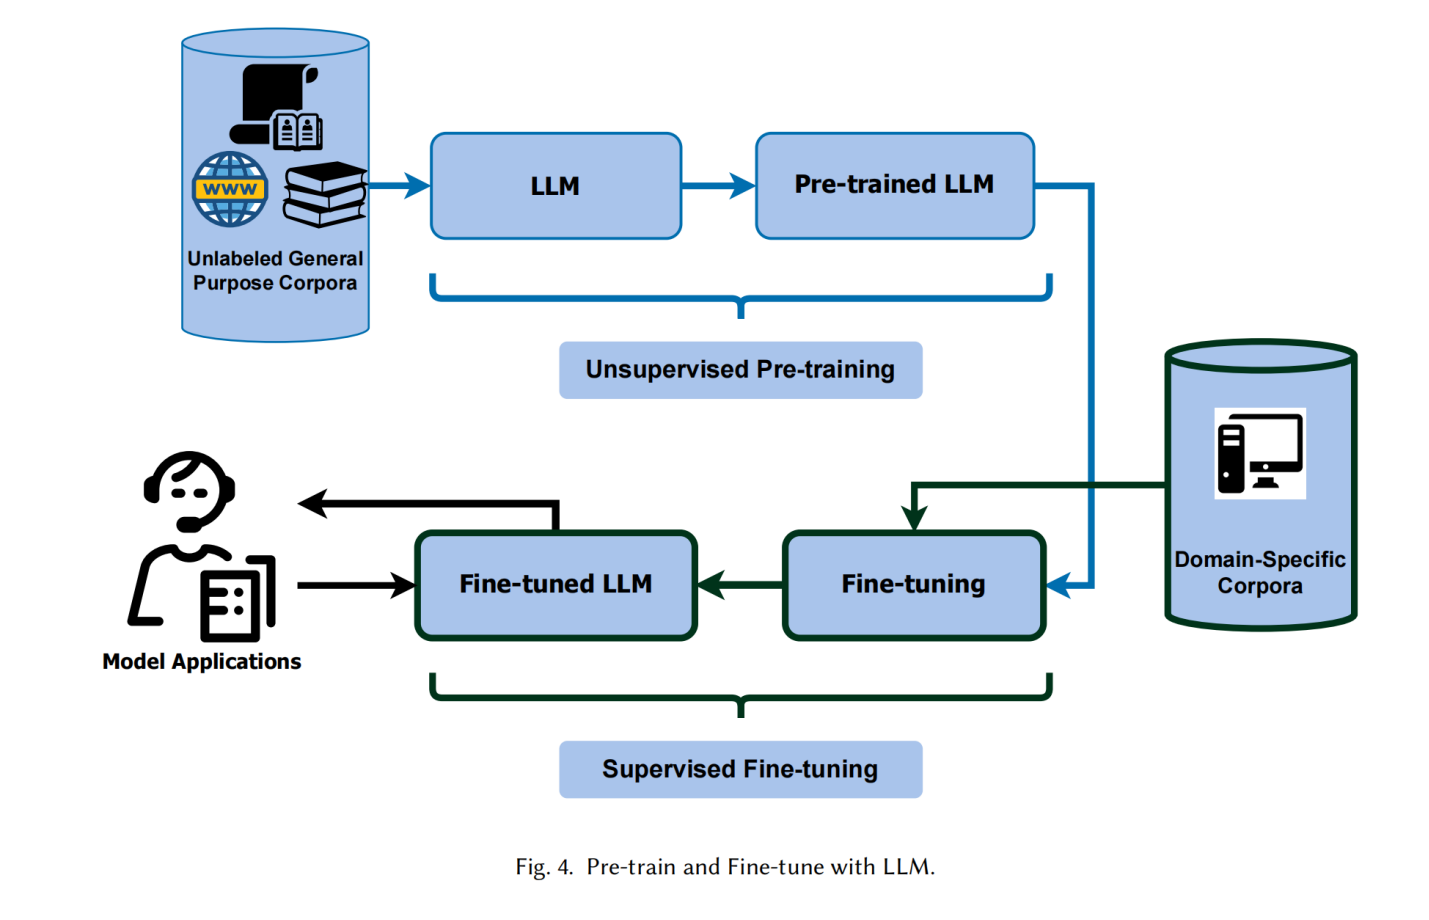
\includegraphics[width=0.8\textwidth]{image2.png}
\caption{预训练与微调范式\protect\footnotemark。}
\label{fig:pretrain}
\end{figure}
\footnotetext{图片来自 Rostam \& Kert\'{e}sz, ACM TIST, 2025, Figure~4。}

核心问题是：在源域上预训练的分类器能否通过在 ST 上微调获得比直接训练更高的 F1？
结果如表~\ref{tab:transfer} 所示。

\begin{table}[htbp]
\centering
\caption{Exp~007 迁移微调核心结果}
\label{tab:transfer}
\small
\begin{tabular}{lccc}
\toprule
\textbf{源域 $\to$ 目标} & \textbf{算法} & \textbf{F1-macro} & \textbf{增益} \\
\midrule
ST $\to$ ST（基线）  & BioBERT+MLP & 0.8345 & --- \\
\textbf{PML $\to$ ST} & \textbf{BioBERT+MLP} & \textbf{0.9143} & \textbf{+9.6\%} \\
OHSUMED $\to$ ST     & BioBERT+MLP & 0.8503 & +1.9\% \\
ST k-NN 图           & GCN          & 0.7716 & --- \\
ST k-NN 图           & GraphSAGE    & 0.7603 & --- \\
\bottomrule
\end{tabular}
\end{table}

\textbf{PML 预训练 + ST 微调达到全场最佳 F1=0.9143}，比直接训练提升 +9.6\%。
源域选择至关重要——PML（16 标签，同类型数据集）的预训练效果远超 OHSUMED
（1,650 标签，异类型，仅 +1.9\%）。
在 ST 上构建 $k$-NN 相似度图后，GCN 和 GraphSAGE 分别达到 0.7716 和 0.7603，
接近 Logistic~Regression 基线但未超越。

\begin{figure}[htbp]
\centering
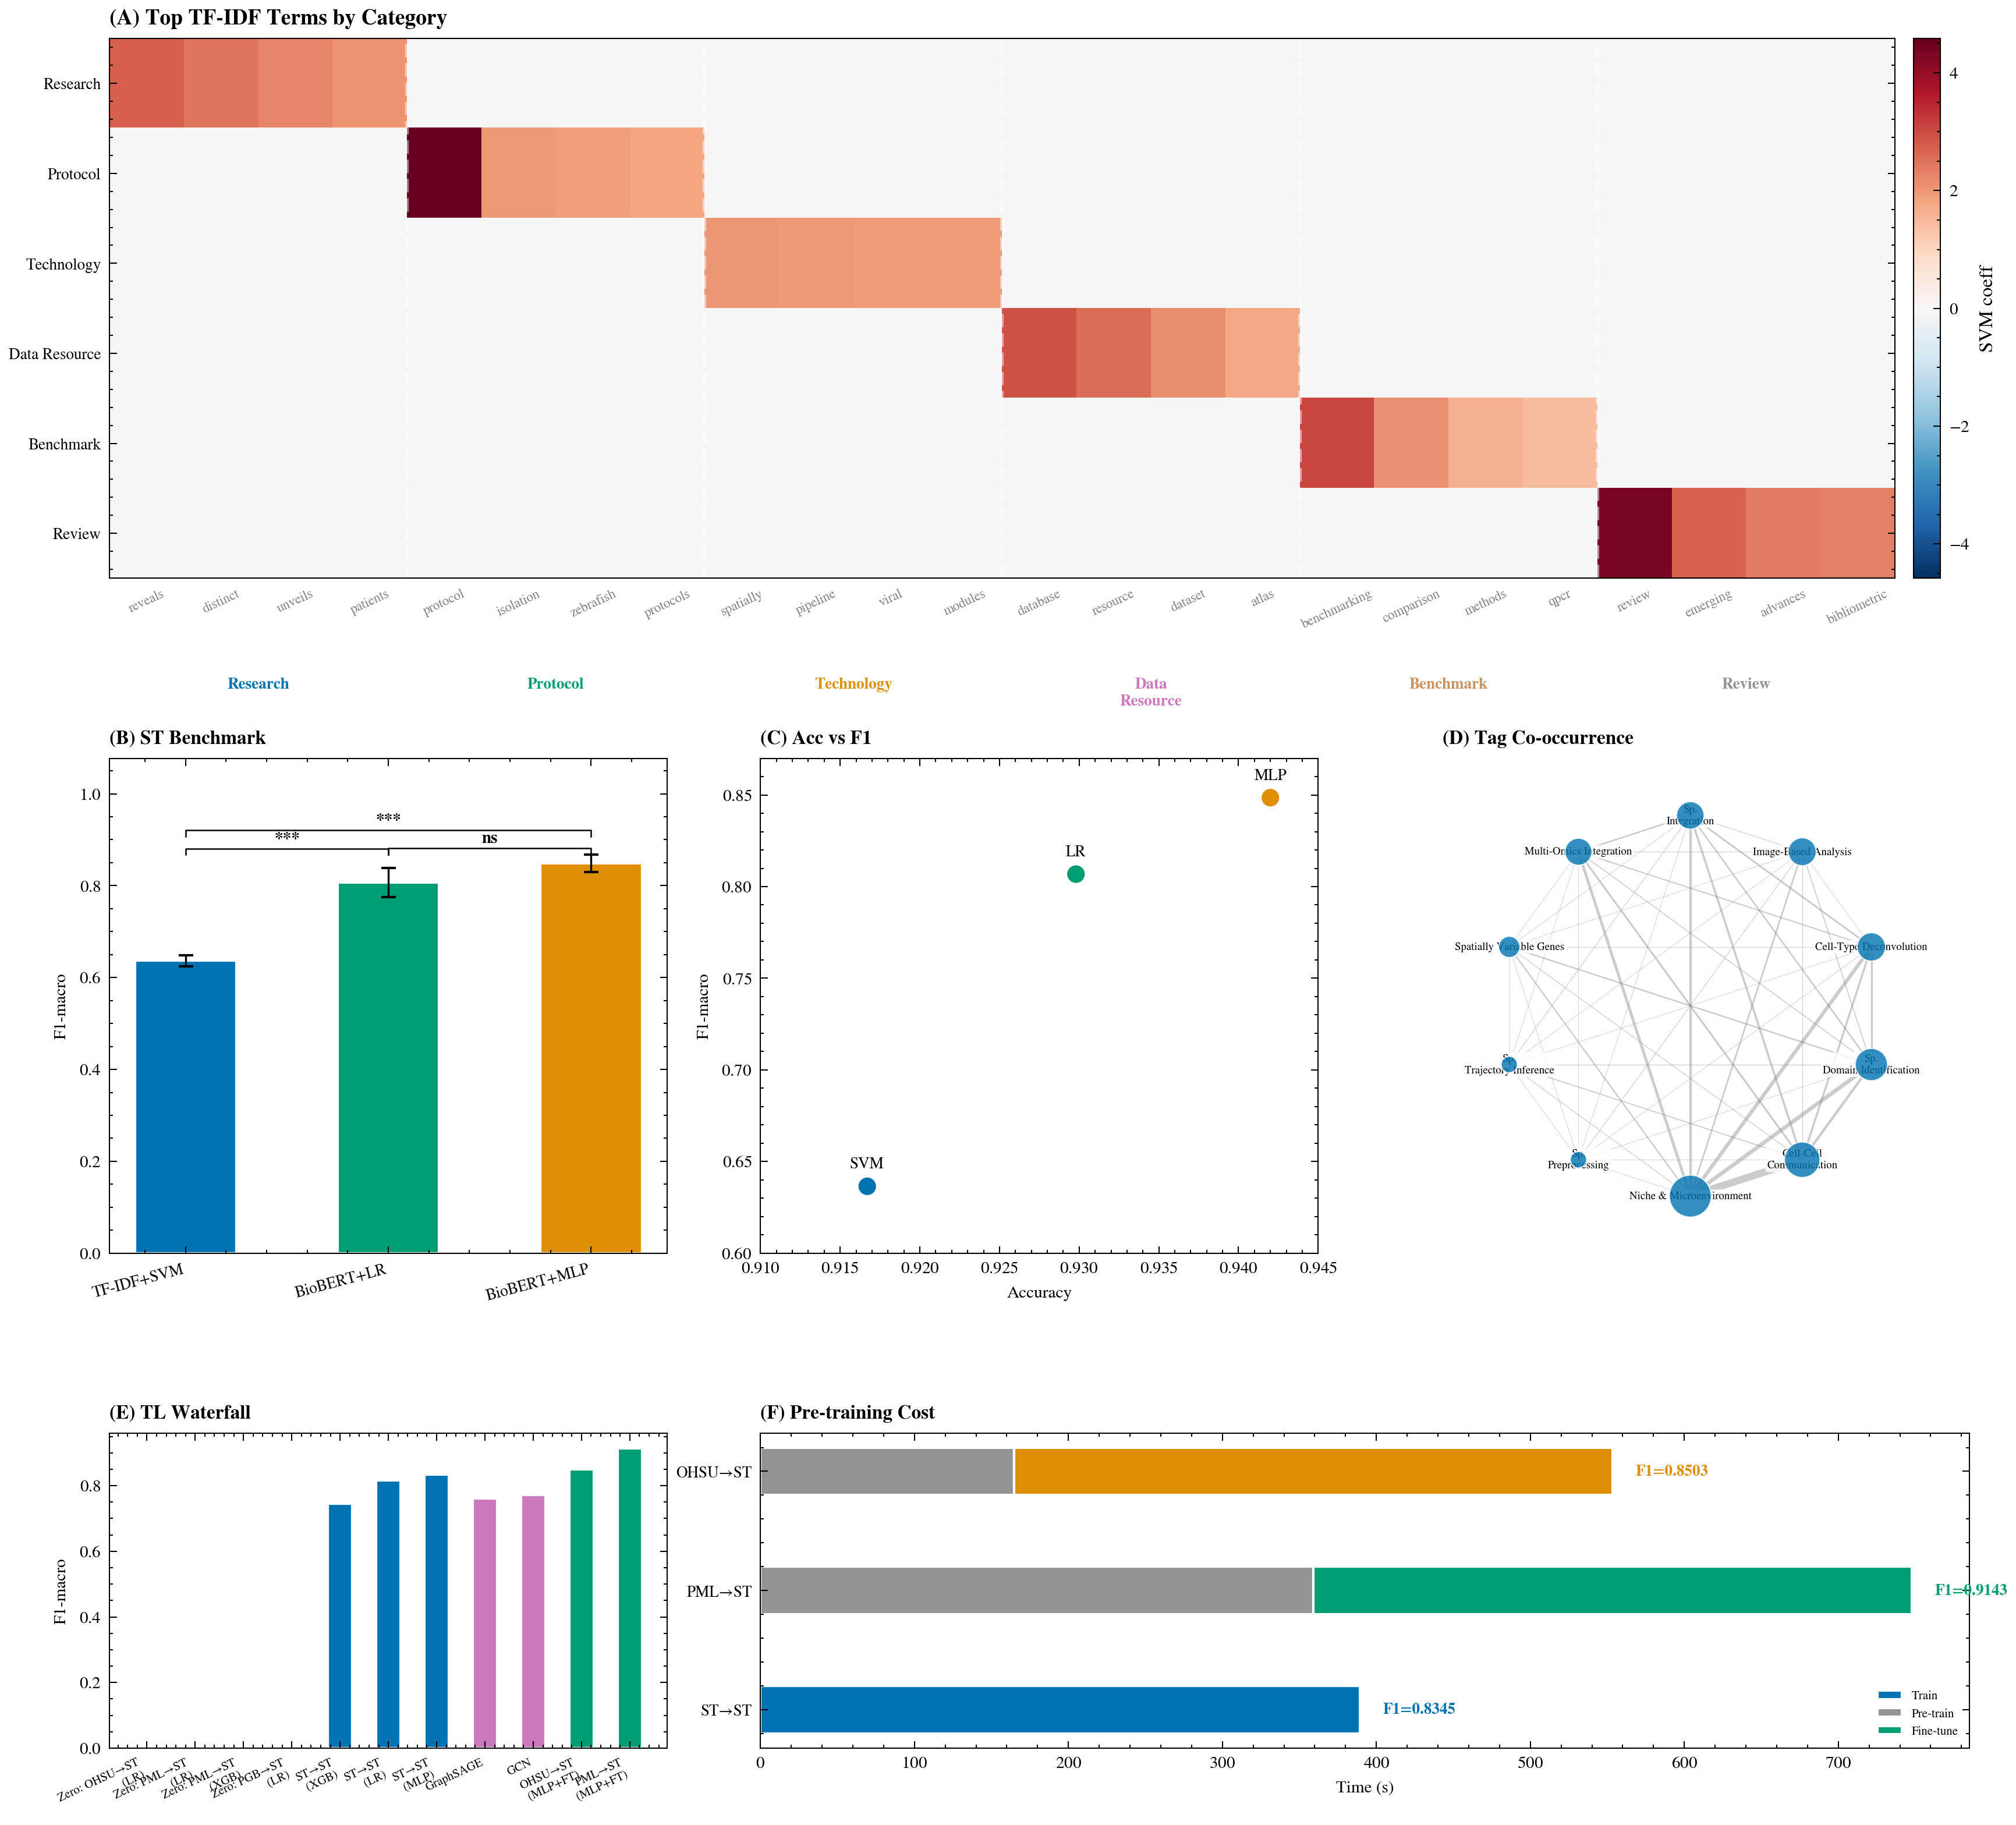
\includegraphics[width=\textwidth]{fig4_st_benchmark_transfer.png}
\caption{ST 基准测试与迁移微调结果。
（A）各类别 Top TF-IDF 词热力图（SVM 系数）；（B）ST 三方法基准测试（含显著性标注）；
（C）Accuracy 与 F1-macro 散点图；（D）Top~10 标签共现网络；
（E）迁移学习瀑布图（零样本~$\to$~基线~$\to$~微调~$\to$~图方法）；
（F）预训练与微调时间成本对比（附 F1 标注）。}
\label{fig:transfer}
\end{figure}

\subsection{嵌入空间可视化}

使用 UMAP 将各数据集的 BioBERT 嵌入投影至二维空间（图~\ref{fig:umap}）。
OHSUMED 因标签空间极其稀疏，所有文献在嵌入空间中聚为单簇；
PML 和 PGB 可见初始的类别分离趋势；
ST 数据集的各类别区分度最好，说明 LLM 标注的标签体系与 BioBERT 嵌入空间高度一致。

\begin{figure}[htbp]
\centering
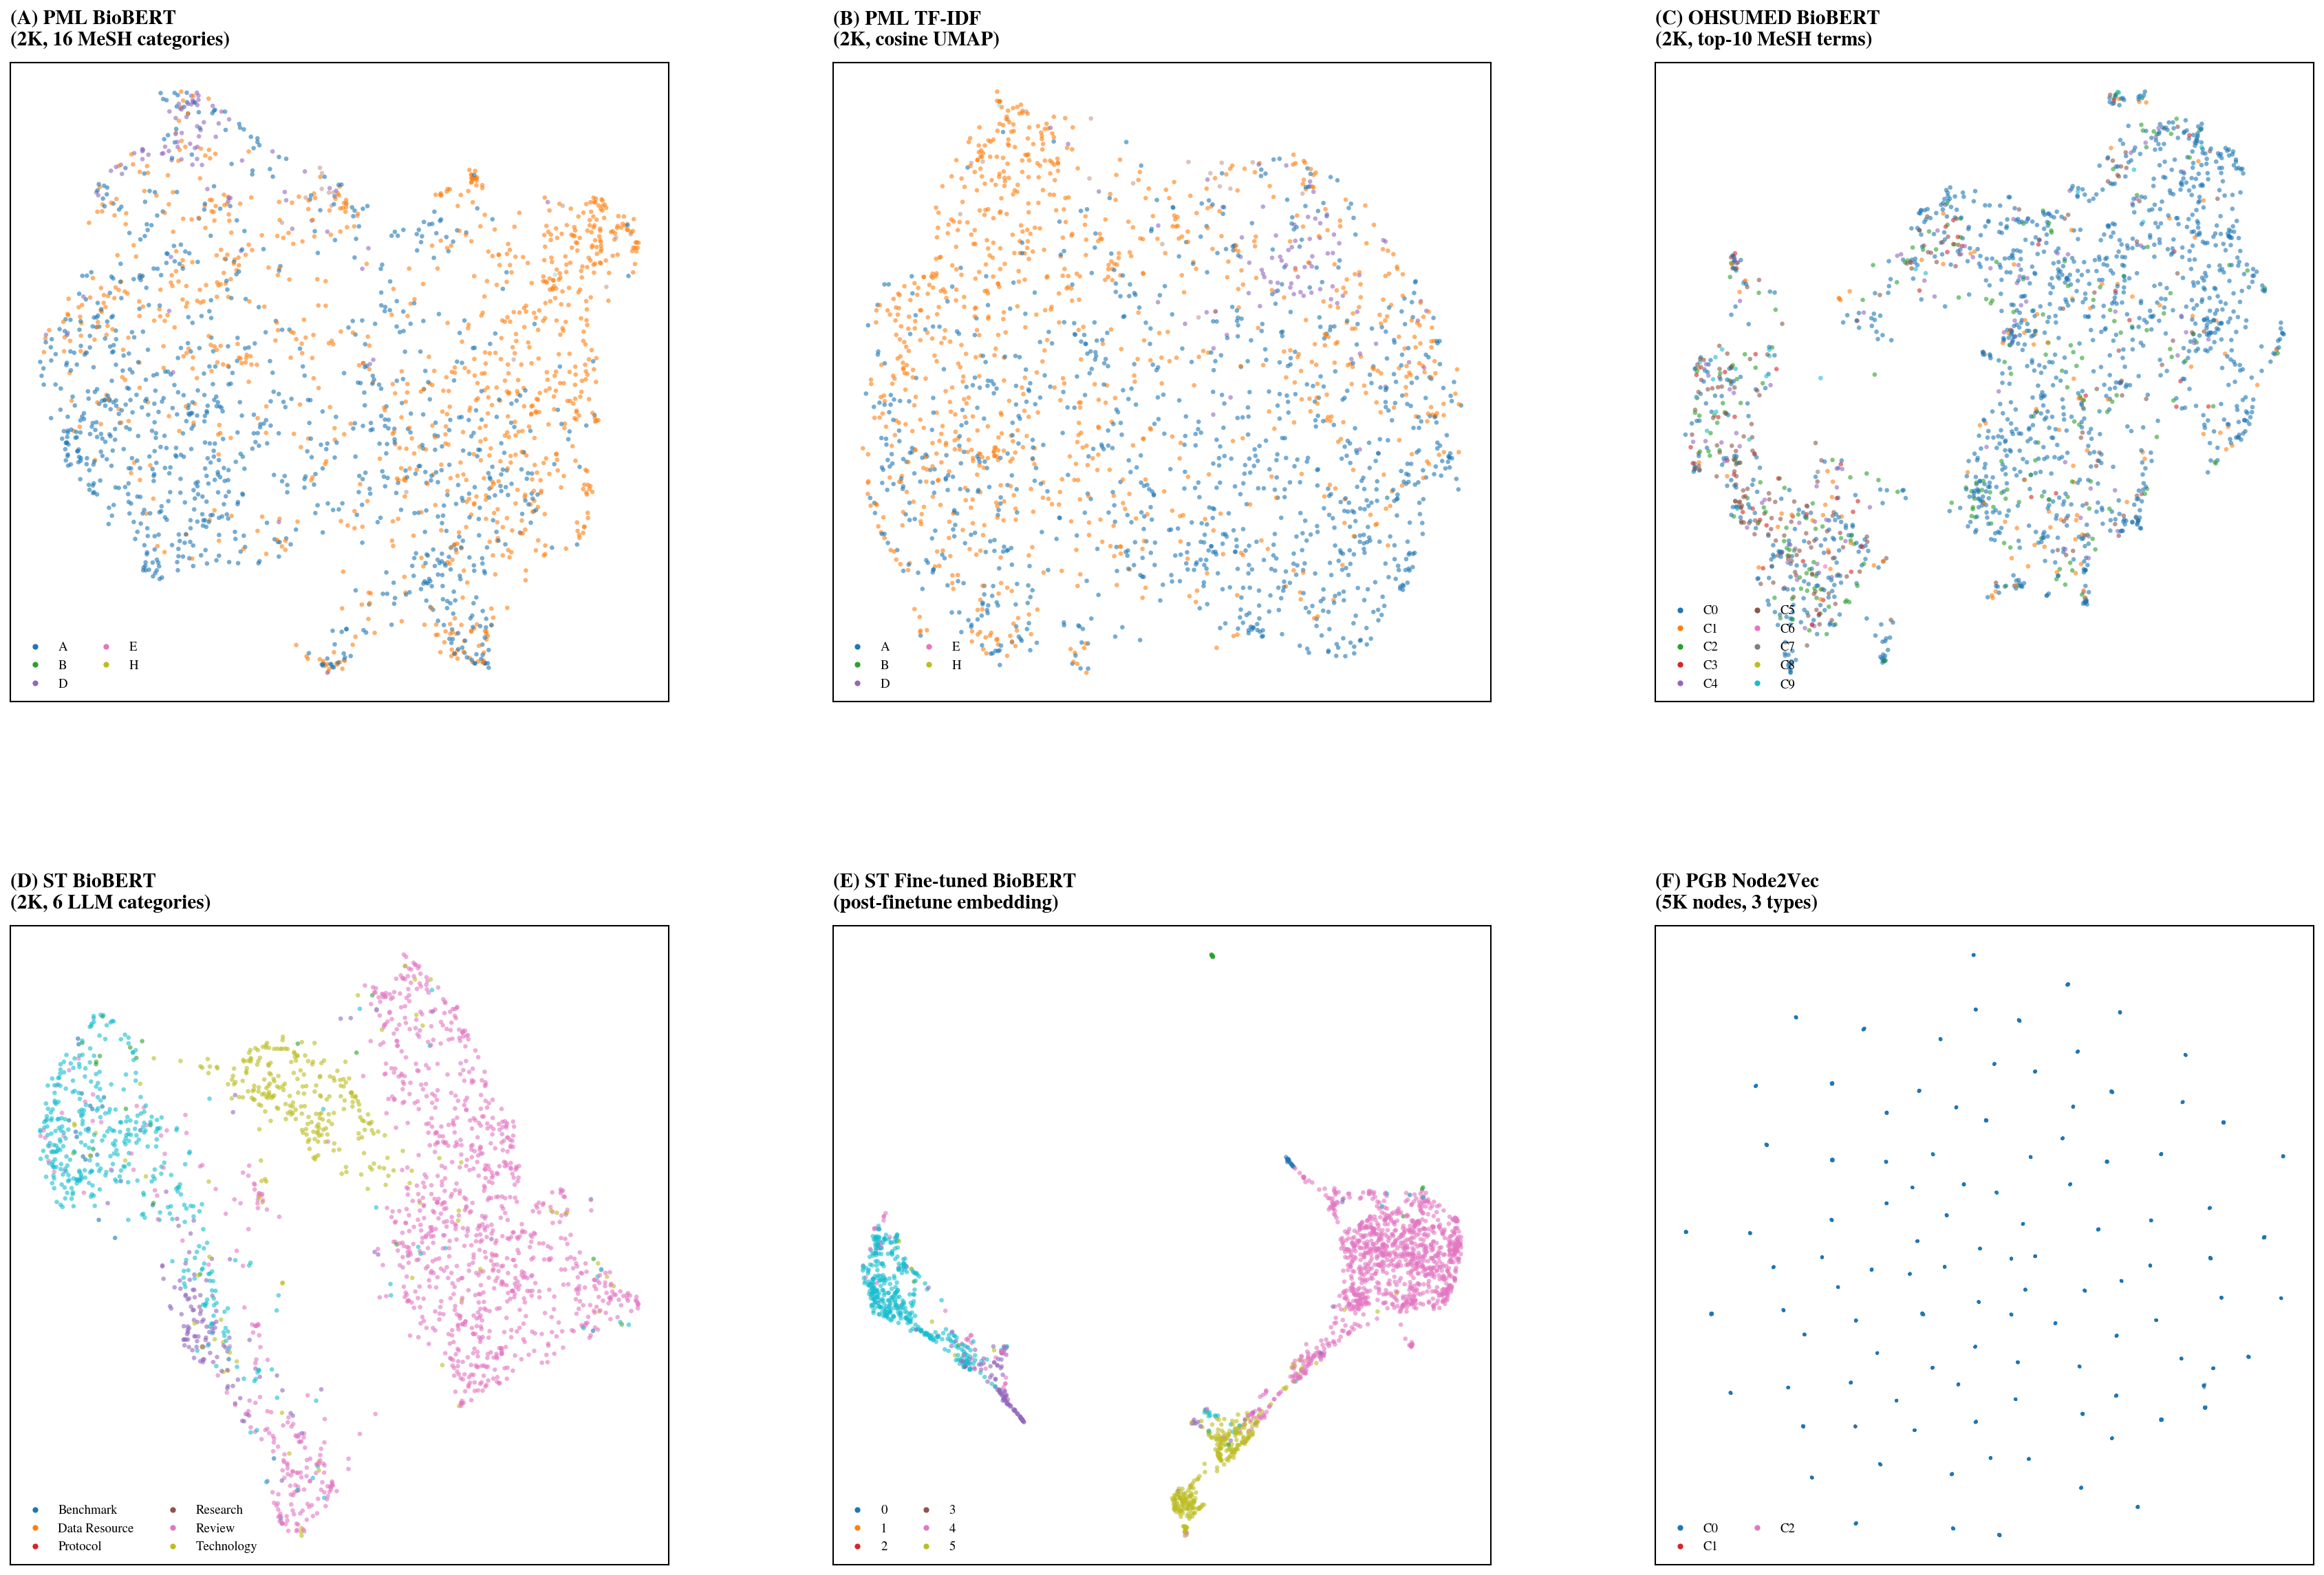
\includegraphics[width=\textwidth]{fig5_umap.png}
\caption{UMAP 嵌入可视化。（A）PML BioBERT 嵌入（2K~点，16~类 MeSH 类别）；
（B）PML TF-IDF 嵌入（2K~点，cosine~距离）；
（C）OHSUMED BioBERT 嵌入（2K~点，Top-10 MeSH 词）；
（D）ST BioBERT 嵌入（2K~点，6~类 LLM 标注类别）；
（E）ST 微调后 BioBERT 嵌入（2K~点）；
（F）PGB Node2Vec 嵌入（5K~节点，3~类）。}
\label{fig:umap}
\end{figure}

% ═══════════════════════════════════════════════════════════════
\section{五、讨论}
% ═══════════════════════════════════════════════════════════════

本文通过 113 组系统实验，得出以下核心发现：

\textbf{(1)~BioBERT 嵌入系统性优于 TF-IDF。}
在所有数据集上，BioBERT 嵌入配合简单分类器（Logistic~Regression）的表现
均优于或等于 TF-IDF 配合复杂模型。说明\textbf{语义深度比特征维度更重要}——
768 维的 BioBERT 嵌入包含的上下文语义信息远超 5,000 维的词袋向量。

\textbf{(2)~标签密度决定算法排序。}
在稠密标签场景（PML，16 类），Logistic~Regression 最优（0.6710）；
在极稀疏标签场景（OHSUMED，1,650 类），AdaBoost 称王（0.1687）。
这一发现提示实际应用中应根据标签密度选择算法。

\textbf{(3)~迁移微调显著有效，源域选择是关键。}
PML 预训练 + ST 微调 F1=0.9143（+9.6\%），而 OHSUMED 预训练仅 +1.9\%。
\textbf{源域与目标域的标签空间结构相似性比源域的数据量更重要}——
PML 的 16 个粗粒度类别与 ST 的 6 个类别在语义结构上更为接近，
而 OHSUMED 的 1,650 个 MeSH 词虽多但粒度差异大。

\textbf{(4)~LLM 批量标注可行性强。}
9,148 篇文献全部由 DeepSeek-v4-flash 自动标注，高置信度和中置信度合计占 95.6\%，
下游分类任务 F1 达到 0.8444--0.9143，说明 LLM 标注质量足以支撑实用的文献分类系统。

\textbf{(5)~GCN 在节点分类上优于随机游走方法。}
在 PGB 上 GCN（0.4125）显著优于 Node2Vec 和 GraphSAGE（均 $\sim$0.3324），
但在 ST 的人工 $k$-NN 图上未能超越 BioBERT+LR 基线，
说明图结构的质量（天然引用图 vs 人工相似度图）对 GCN 性能影响重大。

% ═══════════════════════════════════════════════════════════════
\section{六、结论}
% ═══════════════════════════════════════════════════════════════

本文构建了一个\textbf{多数据集~$\times$~多算法~$\times$~多特征表示}的系统性实验框架，
完成了 7 组实验 113/115 子任务（98.3\%），在 4 个独立数据集上全面比较了 14 种算法、
5 种文本表示和 3 种多标签策略。主要结论如下：

\begin{enumerate}
  \setlength{\itemsep}{-1pt}\setlength{\parsep}{0pt}
  \item BioBERT 嵌入是当前最优的文本表示方法，在所有数据集上系统性优于 TF-IDF。
  \item 算法选择应视标签密度而定：稠密标签用 Logistic~Regression，稀疏标签用 AdaBoost。
  \item PML 预训练 + ST 微调的 BioBERT+MLP 以 F1=0.9143 成为全场最佳方案，
  验证了“宽泛预训练~+~领域微调”范式的有效性，增益达 +9.6\%。
  \item BioBERT+LR 是性价比最优的实用选择（F1=0.8068，138\,s）。
  \item LLM 批量标注在大规模文献分类场景中可行且有效。
\end{enumerate}

\textbf{不足与展望}：(1)~OHSUMED 的 1,650 标签对当前所有方法仍构成挑战，
层次化分类或标签嵌入是潜在改进方向；(2)~图模型在人工 $k$-NN 图上的表现
未超越文本基线，需要探索更优的图构建策略；
(3)~LLM 标注质量的人工抽样评估（Cohen's~$\kappa$）待执行；
(4)~最新研究表明大语言模型在零样本和少样本设定下已接近传统分类器性能\footnote{Proboszcz \& Cichosz, arXiv:2603.11780, 2026}，
将 LLM 作为分类器直接应用于文献标注是值得探索的方向。

\bigskip
\noindent\textbf{参考文献}\\[2pt]
{\small
[1]~Lee \& Ho. PGB: A PubMed Graph Benchmark for Heterogeneous Network Representation Learning. \textit{arXiv:2305.02691}, 2023.\\
[2]~Touchent, Godey \& de~la~Clergerie. Biomed-Enriched: A Biomedical Dataset Enriched with LLMs for Pretraining and Extracting Rare and Hidden Content. \textit{arXiv:2506.20331}, 2025.\\
[3]~Rostam \& Kert\'{e}sz. Advances in Pre-trained Language Models for Domain-Specific Text Classification: A Systematic Review. \textit{ACM Trans. Intell. Syst. Technol.}, 16(6), 2025.\\
[4]~Sakai \& Lam. Large Language Models for Healthcare Text Classification: A Systematic Review. \textit{arXiv:2503.01159}, 2025.\\
[5]~Proboszcz \& Cichosz. Large Language Models for Biomedical Article Classification. \textit{arXiv:2603.11780}, 2026.\\
[6]~Chen et al. Multi-label classification for biomedical literature: an overview of the BioCreative VII LitCovid Track. \textit{Database}, 2022.\\
[7]~Lee et al. BioBERT: a pre-trained biomedical language representation model for biomedical text mining. \textit{Bioinformatics}, 36(4), 2020.\\
}

\bigskip

\noindent\textbf{AI~辅助编程声明：}
本项目全程由 GitHub Copilot 辅助完成，包括代码编写、调试、文档撰写和报告排版。
Copilot 调用的底层模型包括 OpenAI 和 DeepSeek 的 API。
作者本人完成的工作包括：项目整体架构设计、实验方案设计、超参数选择、
结果分析与结论提炼。

\bigskip
\noindent\textbf{数据标注声明：}
空间转录组学文献的 6 维标签体系由作者设计，
批量标注通过 DeepSeek-v4-flash API 调用完成。

\end{document}
